\documentclass[twoside]{book}

% Packages required by doxygen
\usepackage{calc}
\usepackage{doxygen}
\usepackage{graphicx}
\usepackage[utf8]{inputenc}
\usepackage{makeidx}
\usepackage{multicol}
\usepackage{multirow}
\usepackage{textcomp}
\usepackage[table]{xcolor}

% Font selection
\usepackage[T1]{fontenc}
\usepackage{mathptmx}
\usepackage[scaled=.90]{helvet}
\usepackage{courier}
\usepackage{amssymb}
\usepackage{sectsty}
\renewcommand{\familydefault}{\sfdefault}
\allsectionsfont{%
  \fontseries{bc}\selectfont%
  \color{darkgray}%
}
\renewcommand{\DoxyLabelFont}{%
  \fontseries{bc}\selectfont%
  \color{darkgray}%
}

% Page & text layout
\usepackage{geometry}
\geometry{%
  a4paper,%
  top=2.5cm,%
  bottom=2.5cm,%
  left=2.5cm,%
  right=2.5cm%
}
\tolerance=750
\hfuzz=15pt
\hbadness=750
\setlength{\emergencystretch}{15pt}
\setlength{\parindent}{0cm}
\setlength{\parskip}{0.2cm}
\makeatletter
\renewcommand{\paragraph}{%
  \@startsection{paragraph}{4}{0ex}{-1.0ex}{1.0ex}{%
    \normalfont\normalsize\bfseries\SS@parafont%
  }%
}
\renewcommand{\subparagraph}{%
  \@startsection{subparagraph}{5}{0ex}{-1.0ex}{1.0ex}{%
    \normalfont\normalsize\bfseries\SS@subparafont%
  }%
}
\makeatother

% Headers & footers
\usepackage{fancyhdr}
\pagestyle{fancyplain}
\fancyhead[LE]{\fancyplain{}{\bfseries\thepage}}
\fancyhead[CE]{\fancyplain{}{}}
\fancyhead[RE]{\fancyplain{}{\bfseries\leftmark}}
\fancyhead[LO]{\fancyplain{}{\bfseries\rightmark}}
\fancyhead[CO]{\fancyplain{}{}}
\fancyhead[RO]{\fancyplain{}{\bfseries\thepage}}
\fancyfoot[LE]{\fancyplain{}{}}
\fancyfoot[CE]{\fancyplain{}{}}
\fancyfoot[RE]{\fancyplain{}{\bfseries\scriptsize Generated on Fri May 12 2017 02\-:23\-:48 for Turtlebot Lawn Mower by Doxygen }}
\fancyfoot[LO]{\fancyplain{}{\bfseries\scriptsize Generated on Fri May 12 2017 02\-:23\-:48 for Turtlebot Lawn Mower by Doxygen }}
\fancyfoot[CO]{\fancyplain{}{}}
\fancyfoot[RO]{\fancyplain{}{}}
\renewcommand{\footrulewidth}{0.4pt}
\renewcommand{\chaptermark}[1]{%
  \markboth{#1}{}%
}
\renewcommand{\sectionmark}[1]{%
  \markright{\thesection\ #1}%
}

% Indices & bibliography
\usepackage{natbib}
\usepackage[titles]{tocloft}
\setcounter{tocdepth}{3}
\setcounter{secnumdepth}{5}
\makeindex

% Hyperlinks (required, but should be loaded last)
\usepackage{ifpdf}
\ifpdf
  \usepackage[pdftex,pagebackref=true]{hyperref}
\else
  \usepackage[ps2pdf,pagebackref=true]{hyperref}
\fi
\hypersetup{%
  colorlinks=true,%
  linkcolor=blue,%
  citecolor=blue,%
  unicode%
}

% Custom commands
\newcommand{\clearemptydoublepage}{%
  \newpage{\pagestyle{empty}\cleardoublepage}%
}


%===== C O N T E N T S =====

\begin{document}

% Titlepage & ToC
\hypersetup{pageanchor=false}
\pagenumbering{roman}
\begin{titlepage}
\vspace*{7cm}
\begin{center}%
{\Large Turtlebot Lawn Mower \\[1ex]\large 1.\-0 }\\
\vspace*{1cm}
{\large Generated by Doxygen 1.8.6}\\
\vspace*{0.5cm}
{\small Fri May 12 2017 02:23:48}\\
\end{center}
\end{titlepage}
\clearemptydoublepage
\tableofcontents
\clearemptydoublepage
\pagenumbering{arabic}
\hypersetup{pageanchor=true}

%--- Begin generated contents ---
\chapter{Class Index}
\section{Class List}
Here are the classes, structs, unions and interfaces with brief descriptions\-:\begin{DoxyCompactList}
\item\contentsline{section}{\hyperlink{classLawnMower}{Lawn\-Mower} }{\pageref{classLawnMower}}{}
\end{DoxyCompactList}

\chapter{File Index}
\section{File List}
Here is a list of all files with brief descriptions\-:\begin{DoxyCompactList}
\item\contentsline{section}{include/\hyperlink{LawnMower_8h}{Lawn\-Mower.\-h} \\*File containing the Class \hyperlink{classLawnMower}{Lawn\-Mower} }{\pageref{LawnMower_8h}}{}
\item\contentsline{section}{src/\hyperlink{LawnMower_8cpp}{Lawn\-Mower.\-cpp} \\*File implements the class \hyperlink{classLawnMower}{Lawn\-Mower} }{\pageref{LawnMower_8cpp}}{}
\item\contentsline{section}{src/\hyperlink{turtlebot__lawn__mower_8cpp}{turtlebot\-\_\-lawn\-\_\-mower.\-cpp} \\*File containing the main function }{\pageref{turtlebot__lawn__mower_8cpp}}{}
\item\contentsline{section}{test/\hyperlink{turtlebotTest_8cpp}{turtlebot\-Test.\-cpp} \\*File contains tests for the \hyperlink{classLawnMower}{Lawn\-Mower} class }{\pageref{turtlebotTest_8cpp}}{}
\end{DoxyCompactList}

\chapter{Class Documentation}
\hypertarget{classLawnMower}{\section{Lawn\-Mower Class Reference}
\label{classLawnMower}\index{Lawn\-Mower@{Lawn\-Mower}}
}


{\ttfamily \#include $<$Lawn\-Mower.\-h$>$}

\subsection*{Public Member Functions}
\begin{DoxyCompactItemize}
\item 
void \hyperlink{classLawnMower_a522dfba30f16929bbb4fa60af11771b3}{set\-Path\-X} (std\-::vector$<$ double $>$ x)
\begin{DoxyCompactList}\small\item\em Stores the x coordinates of desired lawn mowing pattern. \end{DoxyCompactList}\item 
void \hyperlink{classLawnMower_aa623d7ab5e162524a7c3ee9fe4de8fe1}{set\-Path\-Y} (std\-::vector$<$ double $>$ y)
\begin{DoxyCompactList}\small\item\em Stores the y coordinates of desired lawn mowing pattern. \end{DoxyCompactList}\item 
void \hyperlink{classLawnMower_a05dbed29e3ee522d845c8fbb9fe4b986}{set\-Angle\-Pose} (std\-::vector$<$ double $>$ theta)
\begin{DoxyCompactList}\small\item\em Stores the pose angle of orientation of desired lawn mowing pattern. \end{DoxyCompactList}\item 
void \hyperlink{classLawnMower_af4e360e5861ef467a824c54b3027a25c}{set\-Pose\-Goals} (double x\-Pose, double y\-Pose, geometry\-\_\-msgs\-::\-Quaternion q\-Msg, move\-\_\-base\-\_\-msgs\-::\-Move\-Base\-Goal \&goal)
\begin{DoxyCompactList}\small\item\em Sets a goal coordinate in the x,y plane and pose angle. \end{DoxyCompactList}\item 
void \hyperlink{classLawnMower_ac0a9afe85e5ab7067d1b61d95964119b}{send\-Goal} (move\-\_\-base\-\_\-msgs\-::\-Move\-Base\-Goal goal, actionlib\-::\-Simple\-Action\-Client$<$ move\-\_\-base\-\_\-msgs\-::\-Move\-Base\-Action $>$ \&action\-Client)
\begin{DoxyCompactList}\small\item\em Broadcasts a goal action to the ros network. \end{DoxyCompactList}\item 
tf\-::\-Quaternion \hyperlink{classLawnMower_a97a31ca30db64496d5a85b4218f69cab}{quaternion\-Calculation} (double theta)
\begin{DoxyCompactList}\small\item\em Calculates conversion from Euler angle to Quaternion. \end{DoxyCompactList}\item 
geometry\-\_\-msgs\-::\-Quaternion \hyperlink{classLawnMower_a568bac793e0082f6ff89ac918a671c3b}{convert\-To\-Q\-Msg} (tf\-::\-Quaternion quaternion)
\begin{DoxyCompactList}\small\item\em Converts quaternion to a more suitable message for broadcasting. \end{DoxyCompactList}\item 
const std\-::vector$<$ double $>$ $\ast$ \hyperlink{classLawnMower_a989d400596032888d1e063dc289768b2}{get\-Path\-X\-Coordinate} () const 
\begin{DoxyCompactList}\small\item\em returns specific specified element from x coordinate vector. \end{DoxyCompactList}\item 
const std\-::vector$<$ double $>$ $\ast$ \hyperlink{classLawnMower_a3def1589d73101f642f7465ec740762d}{get\-Path\-Y\-Coordinate} () const 
\begin{DoxyCompactList}\small\item\em returns specific specified element from y coordinate vector. \end{DoxyCompactList}\item 
const std\-::vector$<$ double $>$ $\ast$ \hyperlink{classLawnMower_aec7ea498bca8e6092d7d8ae1f90417c3}{get\-Path\-Angle\-Pose} () const 
\begin{DoxyCompactList}\small\item\em returns specific specified element from pose angle vector. \end{DoxyCompactList}\end{DoxyCompactItemize}


\subsection{Member Function Documentation}
\hypertarget{classLawnMower_a568bac793e0082f6ff89ac918a671c3b}{\index{Lawn\-Mower@{Lawn\-Mower}!convert\-To\-Q\-Msg@{convert\-To\-Q\-Msg}}
\index{convert\-To\-Q\-Msg@{convert\-To\-Q\-Msg}!LawnMower@{Lawn\-Mower}}
\subsubsection[{convert\-To\-Q\-Msg}]{\setlength{\rightskip}{0pt plus 5cm}geometry\-\_\-msgs\-::\-Quaternion Lawn\-Mower\-::convert\-To\-Q\-Msg (
\begin{DoxyParamCaption}
\item[{tf\-::\-Quaternion}]{quaternion}
\end{DoxyParamCaption}
)}}\label{classLawnMower_a568bac793e0082f6ff89ac918a671c3b}


Converts quaternion to a more suitable message for broadcasting. 


\begin{DoxyParams}{Parameters}
{\em quaternion} & quaternion containing goal pose data. \\
\hline
\end{DoxyParams}
\begin{DoxyReturn}{Returns}
geometry\-\_\-msgs\-::\-Quaternion quaternion message that contains goal pose data. 
\end{DoxyReturn}

\begin{DoxyCode}
77 \{
78   geometry\_msgs::Quaternion qMsg;
79   tf::quaternionTFToMsg(quaternion, qMsg);
80   \textcolor{keywordflow}{return} qMsg;
81 \}
\end{DoxyCode}
\hypertarget{classLawnMower_aec7ea498bca8e6092d7d8ae1f90417c3}{\index{Lawn\-Mower@{Lawn\-Mower}!get\-Path\-Angle\-Pose@{get\-Path\-Angle\-Pose}}
\index{get\-Path\-Angle\-Pose@{get\-Path\-Angle\-Pose}!LawnMower@{Lawn\-Mower}}
\subsubsection[{get\-Path\-Angle\-Pose}]{\setlength{\rightskip}{0pt plus 5cm}const std\-::vector$<$double$>$$\ast$ Lawn\-Mower\-::get\-Path\-Angle\-Pose (
\begin{DoxyParamCaption}
{}
\end{DoxyParamCaption}
) const\hspace{0.3cm}{\ttfamily [inline]}}}\label{classLawnMower_aec7ea498bca8e6092d7d8ae1f90417c3}


returns specific specified element from pose angle vector. 


\begin{DoxyParams}{Parameters}
{\em none} & \\
\hline
\end{DoxyParams}
\begin{DoxyReturn}{Returns}
const std\-::vector$<$double$>$$\ast$ pointer to element of pose angle vector. 
\end{DoxyReturn}

\begin{DoxyCode}
109 \{\textcolor{keywordflow}{return} &pathAnglePose;\}
\end{DoxyCode}
\hypertarget{classLawnMower_a989d400596032888d1e063dc289768b2}{\index{Lawn\-Mower@{Lawn\-Mower}!get\-Path\-X\-Coordinate@{get\-Path\-X\-Coordinate}}
\index{get\-Path\-X\-Coordinate@{get\-Path\-X\-Coordinate}!LawnMower@{Lawn\-Mower}}
\subsubsection[{get\-Path\-X\-Coordinate}]{\setlength{\rightskip}{0pt plus 5cm}const std\-::vector$<$double$>$$\ast$ Lawn\-Mower\-::get\-Path\-X\-Coordinate (
\begin{DoxyParamCaption}
{}
\end{DoxyParamCaption}
) const\hspace{0.3cm}{\ttfamily [inline]}}}\label{classLawnMower_a989d400596032888d1e063dc289768b2}


returns specific specified element from x coordinate vector. 


\begin{DoxyParams}{Parameters}
{\em none} & \\
\hline
\end{DoxyParams}
\begin{DoxyReturn}{Returns}
const std\-::vector$<$double$>$$\ast$ pointer to element of x coordinate vector. 
\end{DoxyReturn}

\begin{DoxyCode}
97 \{\textcolor{keywordflow}{return} &pathXCoordinates;\}
\end{DoxyCode}
\hypertarget{classLawnMower_a3def1589d73101f642f7465ec740762d}{\index{Lawn\-Mower@{Lawn\-Mower}!get\-Path\-Y\-Coordinate@{get\-Path\-Y\-Coordinate}}
\index{get\-Path\-Y\-Coordinate@{get\-Path\-Y\-Coordinate}!LawnMower@{Lawn\-Mower}}
\subsubsection[{get\-Path\-Y\-Coordinate}]{\setlength{\rightskip}{0pt plus 5cm}const std\-::vector$<$double$>$$\ast$ Lawn\-Mower\-::get\-Path\-Y\-Coordinate (
\begin{DoxyParamCaption}
{}
\end{DoxyParamCaption}
) const\hspace{0.3cm}{\ttfamily [inline]}}}\label{classLawnMower_a3def1589d73101f642f7465ec740762d}


returns specific specified element from y coordinate vector. 


\begin{DoxyParams}{Parameters}
{\em none} & \\
\hline
\end{DoxyParams}
\begin{DoxyReturn}{Returns}
const std\-::vector$<$double$>$$\ast$ pointer to element of y coordinate vector. 
\end{DoxyReturn}

\begin{DoxyCode}
103 \{\textcolor{keywordflow}{return} &pathYCoordinates;\}
\end{DoxyCode}
\hypertarget{classLawnMower_a97a31ca30db64496d5a85b4218f69cab}{\index{Lawn\-Mower@{Lawn\-Mower}!quaternion\-Calculation@{quaternion\-Calculation}}
\index{quaternion\-Calculation@{quaternion\-Calculation}!LawnMower@{Lawn\-Mower}}
\subsubsection[{quaternion\-Calculation}]{\setlength{\rightskip}{0pt plus 5cm}tf\-::\-Quaternion Lawn\-Mower\-::quaternion\-Calculation (
\begin{DoxyParamCaption}
\item[{double}]{theta}
\end{DoxyParamCaption}
)}}\label{classLawnMower_a97a31ca30db64496d5a85b4218f69cab}


Calculates conversion from Euler angle to Quaternion. 


\begin{DoxyParams}{Parameters}
{\em theta} & pose yaw angle. \\
\hline
\end{DoxyParams}
\begin{DoxyReturn}{Returns}
tf\-::\-Quaternion quaternion containing goal pose data. 
\end{DoxyReturn}

\begin{DoxyCode}
69 \{
70   \textcolor{keywordtype}{double} radians = theta*(M\_PI/180);
71   tf::Quaternion quaternion;
72   quaternion = tf::createQuaternionFromYaw(radians);
73   \textcolor{keywordflow}{return} quaternion;
74 \}
\end{DoxyCode}
\hypertarget{classLawnMower_ac0a9afe85e5ab7067d1b61d95964119b}{\index{Lawn\-Mower@{Lawn\-Mower}!send\-Goal@{send\-Goal}}
\index{send\-Goal@{send\-Goal}!LawnMower@{Lawn\-Mower}}
\subsubsection[{send\-Goal}]{\setlength{\rightskip}{0pt plus 5cm}void Lawn\-Mower\-::send\-Goal (
\begin{DoxyParamCaption}
\item[{move\-\_\-base\-\_\-msgs\-::\-Move\-Base\-Goal}]{goal, }
\item[{actionlib\-::\-Simple\-Action\-Client$<$ move\-\_\-base\-\_\-msgs\-::\-Move\-Base\-Action $>$ \&}]{action\-Client}
\end{DoxyParamCaption}
)}}\label{classLawnMower_ac0a9afe85e5ab7067d1b61d95964119b}


Broadcasts a goal action to the ros network. 


\begin{DoxyParams}{Parameters}
{\em goal} & desired location for turtlebot robot \\
\hline
{\em action\-Client} & Object that broadcasts goal to network \\
\hline
\end{DoxyParams}
\begin{DoxyReturn}{Returns}
void function does not return anything 
\end{DoxyReturn}

\begin{DoxyCode}
63 \{
64   ROS\_INFO(\textcolor{stringliteral}{"Sending robot to:x= %f, y= %f, theta= %f"}, goal.target\_pose.pose.position.x, goal.target\_pose.
      pose.position.y, goal.target\_pose.pose.orientation);
65   actionClient.sendGoal(goal);
66 \}
\end{DoxyCode}
\hypertarget{classLawnMower_a05dbed29e3ee522d845c8fbb9fe4b986}{\index{Lawn\-Mower@{Lawn\-Mower}!set\-Angle\-Pose@{set\-Angle\-Pose}}
\index{set\-Angle\-Pose@{set\-Angle\-Pose}!LawnMower@{Lawn\-Mower}}
\subsubsection[{set\-Angle\-Pose}]{\setlength{\rightskip}{0pt plus 5cm}void Lawn\-Mower\-::set\-Angle\-Pose (
\begin{DoxyParamCaption}
\item[{std\-::vector$<$ double $>$}]{theta}
\end{DoxyParamCaption}
)}}\label{classLawnMower_a05dbed29e3ee522d845c8fbb9fe4b986}


Stores the pose angle of orientation of desired lawn mowing pattern. 


\begin{DoxyParams}{Parameters}
{\em theta} & pose angle of orientation \\
\hline
\end{DoxyParams}
\begin{DoxyReturn}{Returns}
void function does not return anything 
\end{DoxyReturn}

\begin{DoxyCode}
49 \{
50   pathAnglePose = theta;
51 \}
\end{DoxyCode}
\hypertarget{classLawnMower_a522dfba30f16929bbb4fa60af11771b3}{\index{Lawn\-Mower@{Lawn\-Mower}!set\-Path\-X@{set\-Path\-X}}
\index{set\-Path\-X@{set\-Path\-X}!LawnMower@{Lawn\-Mower}}
\subsubsection[{set\-Path\-X}]{\setlength{\rightskip}{0pt plus 5cm}void Lawn\-Mower\-::set\-Path\-X (
\begin{DoxyParamCaption}
\item[{std\-::vector$<$ double $>$}]{x}
\end{DoxyParamCaption}
)}}\label{classLawnMower_a522dfba30f16929bbb4fa60af11771b3}


Stores the x coordinates of desired lawn mowing pattern. 


\begin{DoxyParams}{Parameters}
{\em x} & data coordinates of x axis \\
\hline
\end{DoxyParams}
\begin{DoxyReturn}{Returns}
void function does not return anything 
\end{DoxyReturn}

\begin{DoxyCode}
39 \{
40   pathXCoordinates = x;
41 \}
\end{DoxyCode}
\hypertarget{classLawnMower_aa623d7ab5e162524a7c3ee9fe4de8fe1}{\index{Lawn\-Mower@{Lawn\-Mower}!set\-Path\-Y@{set\-Path\-Y}}
\index{set\-Path\-Y@{set\-Path\-Y}!LawnMower@{Lawn\-Mower}}
\subsubsection[{set\-Path\-Y}]{\setlength{\rightskip}{0pt plus 5cm}void Lawn\-Mower\-::set\-Path\-Y (
\begin{DoxyParamCaption}
\item[{std\-::vector$<$ double $>$}]{y}
\end{DoxyParamCaption}
)}}\label{classLawnMower_aa623d7ab5e162524a7c3ee9fe4de8fe1}


Stores the y coordinates of desired lawn mowing pattern. 


\begin{DoxyParams}{Parameters}
{\em y} & data coordinates of y axis \\
\hline
\end{DoxyParams}
\begin{DoxyReturn}{Returns}
void function does not return anything 
\end{DoxyReturn}

\begin{DoxyCode}
44 \{
45   pathYCoordinates = y;
46 \}
\end{DoxyCode}
\hypertarget{classLawnMower_af4e360e5861ef467a824c54b3027a25c}{\index{Lawn\-Mower@{Lawn\-Mower}!set\-Pose\-Goals@{set\-Pose\-Goals}}
\index{set\-Pose\-Goals@{set\-Pose\-Goals}!LawnMower@{Lawn\-Mower}}
\subsubsection[{set\-Pose\-Goals}]{\setlength{\rightskip}{0pt plus 5cm}void Lawn\-Mower\-::set\-Pose\-Goals (
\begin{DoxyParamCaption}
\item[{double}]{x\-Pose, }
\item[{double}]{y\-Pose, }
\item[{geometry\-\_\-msgs\-::\-Quaternion}]{q\-Msg, }
\item[{move\-\_\-base\-\_\-msgs\-::\-Move\-Base\-Goal \&}]{goal}
\end{DoxyParamCaption}
)}}\label{classLawnMower_af4e360e5861ef467a824c54b3027a25c}


Sets a goal coordinate in the x,y plane and pose angle. 


\begin{DoxyParams}{Parameters}
{\em x\-Pose} & goal x coordinate \\
\hline
{\em y\-Pose} & goal y coordinate \\
\hline
{\em q\-Msg} & quaternion angle pose message \\
\hline
{\em goal} & stores goal coordinates and pose angle \\
\hline
\end{DoxyParams}
\begin{DoxyReturn}{Returns}
void function does not return anything 
\end{DoxyReturn}

\begin{DoxyCode}
54 \{
55   goal.target\_pose.header.frame\_id = \textcolor{stringliteral}{"map"};
56   goal.target\_pose.header.stamp = ros::Time::now();
57   goal.target\_pose.pose.position.x = xPose;
58   goal.target\_pose.pose.position.y = yPose;
59   goal.target\_pose.pose.orientation = qMsg;
60 \}
\end{DoxyCode}


The documentation for this class was generated from the following files\-:\begin{DoxyCompactItemize}
\item 
include/\hyperlink{LawnMower_8h}{Lawn\-Mower.\-h}\item 
src/\hyperlink{LawnMower_8cpp}{Lawn\-Mower.\-cpp}\end{DoxyCompactItemize}

\chapter{File Documentation}
\hypertarget{LawnMower_8h}{\section{include/\-Lawn\-Mower.h File Reference}
\label{LawnMower_8h}\index{include/\-Lawn\-Mower.\-h@{include/\-Lawn\-Mower.\-h}}
}


File containing the Class \hyperlink{classLawnMower}{Lawn\-Mower}.  


{\ttfamily \#include $<$ros/ros.\-h$>$}\\*
{\ttfamily \#include $<$move\-\_\-base\-\_\-msgs/\-Move\-Base\-Action.\-h$>$}\\*
{\ttfamily \#include $<$actionlib/client/simple\-\_\-action\-\_\-client.\-h$>$}\\*
{\ttfamily \#include $<$tf/transform\-\_\-datatypes.\-h$>$}\\*
{\ttfamily \#include $<$vector$>$}\\*
Include dependency graph for Lawn\-Mower.\-h\-:
\nopagebreak
\begin{figure}[H]
\begin{center}
\leavevmode
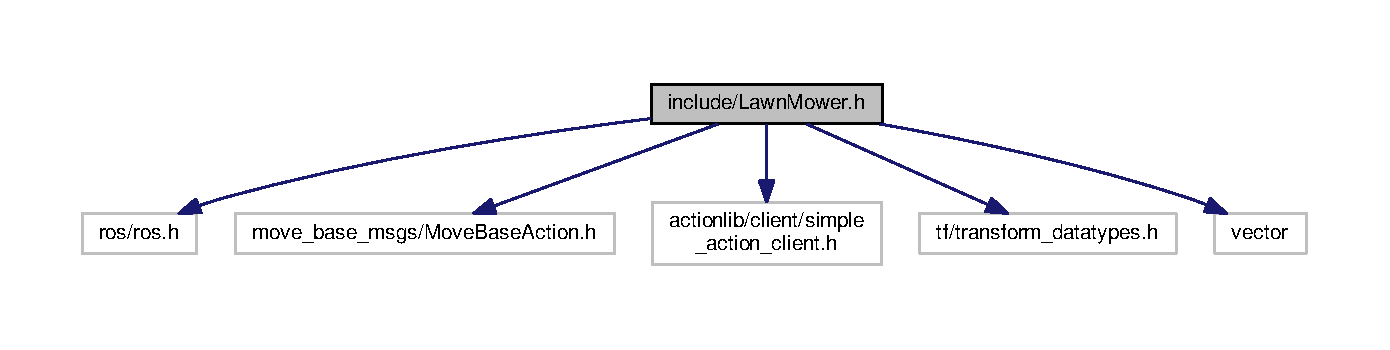
\includegraphics[width=350pt]{LawnMower_8h__incl}
\end{center}
\end{figure}
This graph shows which files directly or indirectly include this file\-:
\nopagebreak
\begin{figure}[H]
\begin{center}
\leavevmode
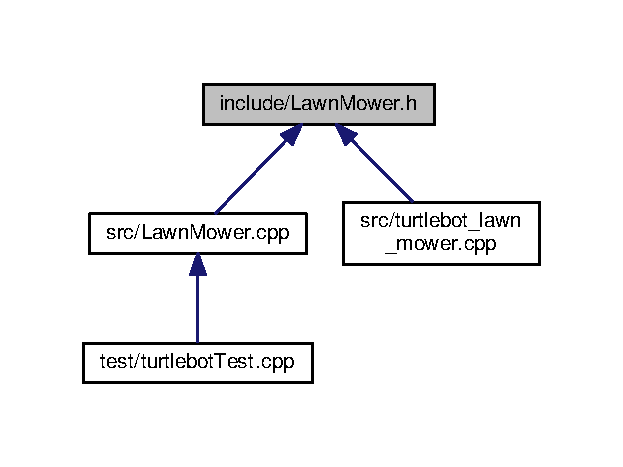
\includegraphics[width=299pt]{LawnMower_8h__dep__incl}
\end{center}
\end{figure}
\subsection*{Classes}
\begin{DoxyCompactItemize}
\item 
class \hyperlink{classLawnMower}{Lawn\-Mower}
\end{DoxyCompactItemize}


\subsection{Detailed Description}
File containing the Class \hyperlink{classLawnMower}{Lawn\-Mower}. \begin{DoxyAuthor}{Author}
Christian Ramos 
\end{DoxyAuthor}
\begin{DoxyDate}{Date}
8 May 2017 The class \hyperlink{classLawnMower}{Lawn\-Mower} stores coordinates that the turtlebot robot will follow in order to acomplished its lawn mowing task. This class also creates goals based on the coordinates data and controls the robot path along the backyard simulated field in the gazebo simulator. 
\end{DoxyDate}
\begin{DoxySeeAlso}{See Also}
\href{https://github.com/traviezo/turtlebot_lawn_mower}{\tt https\-://github.\-com/traviezo/turtlebot\-\_\-lawn\-\_\-mower} 
\end{DoxySeeAlso}

\hypertarget{LawnMower_8cpp}{\section{src/\-Lawn\-Mower.cpp File Reference}
\label{LawnMower_8cpp}\index{src/\-Lawn\-Mower.\-cpp@{src/\-Lawn\-Mower.\-cpp}}
}


File implements the class \hyperlink{classLawnMower}{Lawn\-Mower}.  


{\ttfamily \#include \char`\"{}../include/\-Lawn\-Mower.\-h\char`\"{}}\\*
{\ttfamily \#include $<$vector$>$}\\*
Include dependency graph for Lawn\-Mower.\-cpp\-:
\nopagebreak
\begin{figure}[H]
\begin{center}
\leavevmode
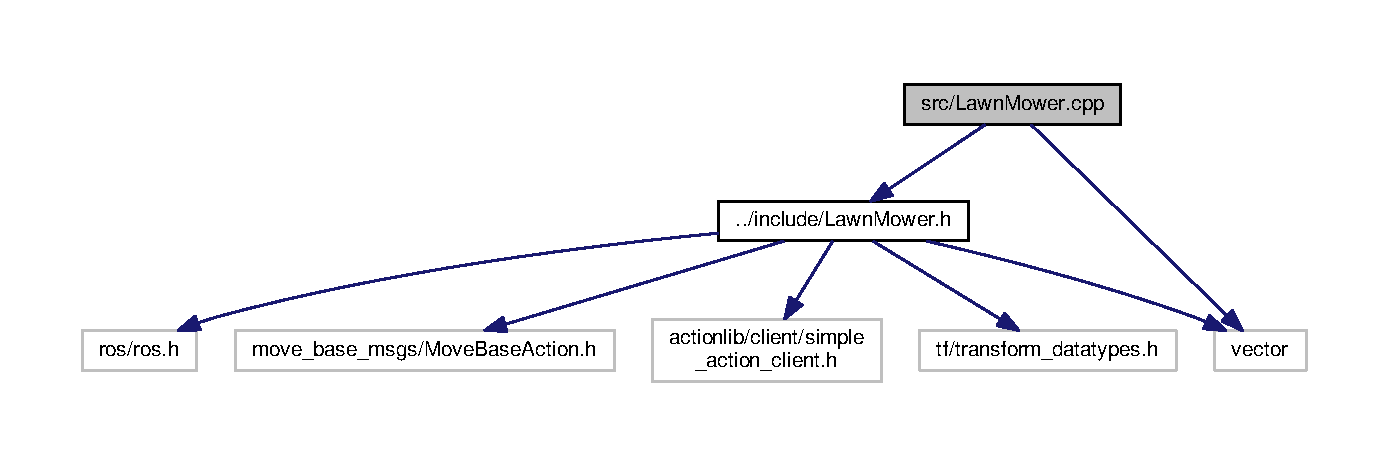
\includegraphics[width=350pt]{LawnMower_8cpp__incl}
\end{center}
\end{figure}
This graph shows which files directly or indirectly include this file\-:
\nopagebreak
\begin{figure}[H]
\begin{center}
\leavevmode
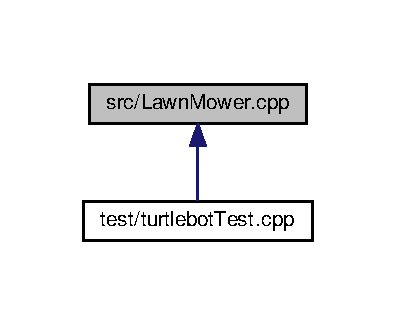
\includegraphics[width=190pt]{LawnMower_8cpp__dep__incl}
\end{center}
\end{figure}


\subsection{Detailed Description}
File implements the class \hyperlink{classLawnMower}{Lawn\-Mower}. \begin{DoxyAuthor}{Author}
Christian Ramos 
\end{DoxyAuthor}
\begin{DoxyDate}{Date}
8 May 2017 This file implements all member functions declared in \hyperlink{classLawnMower}{Lawn\-Mower} header file.
\end{DoxyDate}
\begin{DoxySeeAlso}{See Also}
\href{https://github.com/traviezo/turtlebot_lawn_mower}{\tt https\-://github.\-com/traviezo/turtlebot\-\_\-lawn\-\_\-mower} 
\end{DoxySeeAlso}

\hypertarget{turtlebot__lawn__mower_8cpp}{\section{src/turtlebot\-\_\-lawn\-\_\-mower.cpp File Reference}
\label{turtlebot__lawn__mower_8cpp}\index{src/turtlebot\-\_\-lawn\-\_\-mower.\-cpp@{src/turtlebot\-\_\-lawn\-\_\-mower.\-cpp}}
}


File containing the main function.  


{\ttfamily \#include $<$vector$>$}\\*
{\ttfamily \#include \char`\"{}../include/\-Lawn\-Mower.\-h\char`\"{}}\\*
Include dependency graph for turtlebot\-\_\-lawn\-\_\-mower.\-cpp\-:
\nopagebreak
\begin{figure}[H]
\begin{center}
\leavevmode
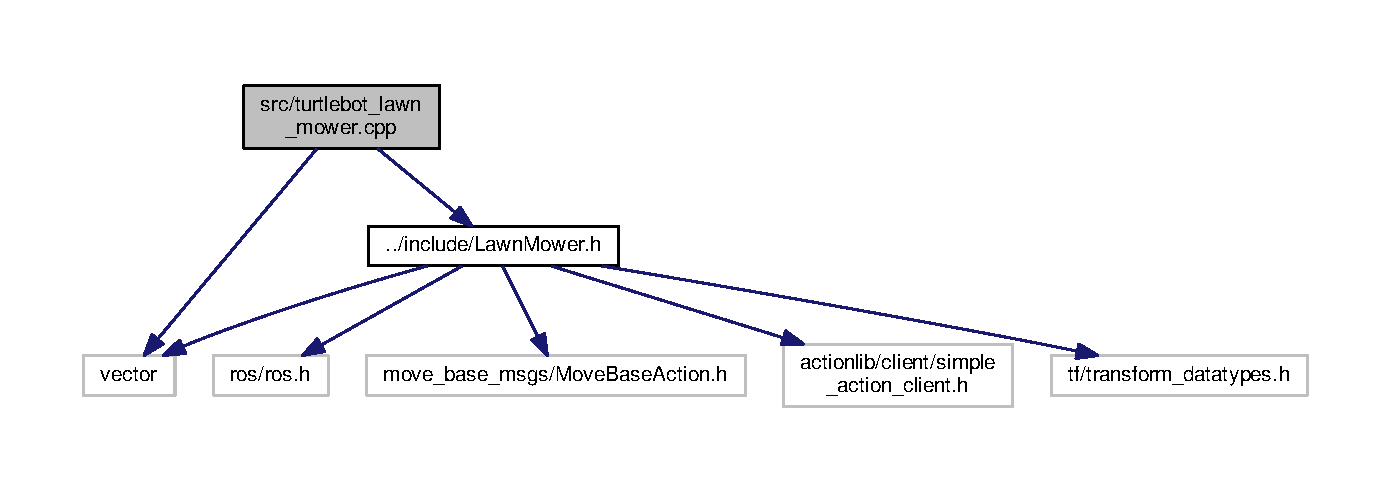
\includegraphics[width=350pt]{turtlebot__lawn__mower_8cpp__incl}
\end{center}
\end{figure}
\subsection*{Typedefs}
\begin{DoxyCompactItemize}
\item 
typedef \\*
actionlib\-::\-Simple\-Action\-Client\\*
$<$ move\-\_\-base\-\_\-msgs\-::\-Move\-Base\-Action $>$ \hyperlink{turtlebot__lawn__mower_8cpp_a21e20cc0b6656ae897b3cbb969b93241}{Move\-Base\-Client}
\end{DoxyCompactItemize}
\subsection*{Functions}
\begin{DoxyCompactItemize}
\item 
int \hyperlink{turtlebot__lawn__mower_8cpp_a3c04138a5bfe5d72780bb7e82a18e627}{main} (int argc, char $\ast$$\ast$argv)
\end{DoxyCompactItemize}
\subsection*{Variables}
\begin{DoxyCompactItemize}
\item 
std\-::vector$<$ double $>$ \hyperlink{turtlebot__lawn__mower_8cpp_ab924092e01ea1007f9b6d88bc3d9c723}{x\-Coordinates} \{ 0.\-25, 0.\-25, 2.\-75, 2.\-75, -\/1.\-25, -\/1.\-25, 3.\-25, 3.\-25, -\/1.\-25, -\/1.\-25, 3.\-25, 3.\-25, -\/1.\-25, -\/1.\-25, 3.\-25, 3.\-25, -\/1.\-25, -\/1.\-25, 3.\-25, 3.\-25, -\/0.\-5, -\/1.\-25, 3.\-25, 3.\-25\}
\item 
std\-::vector$<$ double $>$ \hyperlink{turtlebot__lawn__mower_8cpp_a2fdc9aef0350032e97be2faac7fc0ec8}{y\-Coordinates} \{ 4.\-25, 3.\-75, 3.\-75, 3.\-25, 3.\-25, 2.\-75, 2.\-75, 2.\-25, 2.\-25, 1.\-75, 1.\-75, 1.\-25, 1.\-25, 0.\-75, 0.\-75, 0.\-25, 0.\-25, -\/0.\-25, -\/0.\-25, -\/0.\-5, -\/1.\-5, -\/0.\-25, 4.\-25, 4.\-25\}
\item 
std\-::vector$<$ double $>$ \hyperlink{turtlebot__lawn__mower_8cpp_a06c7ee380c5c4448f42b667fb3a645c4}{angle\-Pose} \{-\/90.\-0, 0.\-0, -\/90.\-0, 180.\-0, -\/90.\-0, 0.\-0, -\/90.\-0, 180, -\/90.\-0, 0.\-0, -\/90.\-0, 180, -\/90.\-0, 0.\-0, -\/90.\-0, 180, -\/90.\-0, 0.\-0, -\/90.\-0, 180.\-0, 90.\-0, 0.\-0, 0.\-0, 180.\-0\}
\item 
int const \hyperlink{turtlebot__lawn__mower_8cpp_a1d25959ca5224ef5554a5605ac902c5d}{N\-U\-M\-B\-E\-R\-\_\-\-O\-F\-\_\-\-G\-O\-A\-L\-\_\-\-P\-O\-S\-E\-S} = 24
\end{DoxyCompactItemize}


\subsection{Detailed Description}
File containing the main function. \begin{DoxyAuthor}{Author}
Christian Ramos 
\end{DoxyAuthor}
\begin{DoxyDate}{Date}
5 May 2017 This file calls the \hyperlink{classLawnMower}{Lawn\-Mower} class and other classes in order to guide the turtlebot along the simulated gazebo world.
\end{DoxyDate}
\begin{DoxySeeAlso}{See Also}
\href{https://github.com/traviezo/turtlebot_lawn_mower}{\tt https\-://github.\-com/traviezo/turtlebot\-\_\-lawn\-\_\-mower} 
\end{DoxySeeAlso}


\subsection{Typedef Documentation}
\hypertarget{turtlebot__lawn__mower_8cpp_a21e20cc0b6656ae897b3cbb969b93241}{\index{turtlebot\-\_\-lawn\-\_\-mower.\-cpp@{turtlebot\-\_\-lawn\-\_\-mower.\-cpp}!Move\-Base\-Client@{Move\-Base\-Client}}
\index{Move\-Base\-Client@{Move\-Base\-Client}!turtlebot_lawn_mower.cpp@{turtlebot\-\_\-lawn\-\_\-mower.\-cpp}}
\subsubsection[{Move\-Base\-Client}]{\setlength{\rightskip}{0pt plus 5cm}typedef actionlib\-::\-Simple\-Action\-Client$<$move\-\_\-base\-\_\-msgs\-::\-Move\-Base\-Action$>$ {\bf Move\-Base\-Client}}}\label{turtlebot__lawn__mower_8cpp_a21e20cc0b6656ae897b3cbb969b93241}


\subsection{Function Documentation}
\hypertarget{turtlebot__lawn__mower_8cpp_a3c04138a5bfe5d72780bb7e82a18e627}{\index{turtlebot\-\_\-lawn\-\_\-mower.\-cpp@{turtlebot\-\_\-lawn\-\_\-mower.\-cpp}!main@{main}}
\index{main@{main}!turtlebot_lawn_mower.cpp@{turtlebot\-\_\-lawn\-\_\-mower.\-cpp}}
\subsubsection[{main}]{\setlength{\rightskip}{0pt plus 5cm}int main (
\begin{DoxyParamCaption}
\item[{int}]{argc, }
\item[{char $\ast$$\ast$}]{argv}
\end{DoxyParamCaption}
)}}\label{turtlebot__lawn__mower_8cpp_a3c04138a5bfe5d72780bb7e82a18e627}

\begin{DoxyCode}
46                                 \{
47   ros::init(argc, argv, \textcolor{stringliteral}{"turtlebot\_lawn\_mower\_node"});
48   ros::NodeHandle nh;
49   \hyperlink{classLawnMower}{LawnMower} lawnMowerBot;
50   move\_base\_msgs::MoveBaseGoal goal;
51   \hyperlink{turtlebot__lawn__mower_8cpp_a21e20cc0b6656ae897b3cbb969b93241}{MoveBaseClient} actionClient(\textcolor{stringliteral}{"move\_base"}, \textcolor{keyword}{true});
52   ROS\_INFO(\textcolor{stringliteral}{"Waiting for the move\_base action server..."});
53   actionClient.waitForServer(ros::Duration(60));
54   ROS\_INFO(\textcolor{stringliteral}{"Connected to move\_base server"});
55   lawnMowerBot.\hyperlink{classLawnMower_a522dfba30f16929bbb4fa60af11771b3}{setPathX}(\hyperlink{turtlebot__lawn__mower_8cpp_ab924092e01ea1007f9b6d88bc3d9c723}{xCoordinates});
56   lawnMowerBot.\hyperlink{classLawnMower_aa623d7ab5e162524a7c3ee9fe4de8fe1}{setPathY}(\hyperlink{turtlebot__lawn__mower_8cpp_a2fdc9aef0350032e97be2faac7fc0ec8}{yCoordinates});
57   lawnMowerBot.\hyperlink{classLawnMower_a05dbed29e3ee522d845c8fbb9fe4b986}{setAnglePose}(\hyperlink{turtlebot__lawn__mower_8cpp_a06c7ee380c5c4448f42b667fb3a645c4}{anglePose});
58   \textcolor{keywordflow}{for} (\textcolor{keywordtype}{int} i = 0; i < \hyperlink{turtlebot__lawn__mower_8cpp_a1d25959ca5224ef5554a5605ac902c5d}{NUMBER\_OF\_GOAL\_POSES}; i++) \{
59     tf::Quaternion quaternion;
60     quaternion = lawnMowerBot.\hyperlink{classLawnMower_a97a31ca30db64496d5a85b4218f69cab}{quaternionCalculation}(lawnMowerBot.
      \hyperlink{classLawnMower_aec7ea498bca8e6092d7d8ae1f90417c3}{getPathAnglePose}()->at(i));
61     geometry\_msgs::Quaternion qMsg;
62     qMsg = lawnMowerBot.\hyperlink{classLawnMower_a568bac793e0082f6ff89ac918a671c3b}{convertToQMsg}(quaternion);
63     lawnMowerBot.\hyperlink{classLawnMower_af4e360e5861ef467a824c54b3027a25c}{setPoseGoals}(lawnMowerBot.\hyperlink{classLawnMower_a989d400596032888d1e063dc289768b2}{getPathXCoordinate}()->at(i), 
      lawnMowerBot.\hyperlink{classLawnMower_a3def1589d73101f642f7465ec740762d}{getPathYCoordinate}()->at(i), qMsg, goal);
64     lawnMowerBot.\hyperlink{classLawnMower_ac0a9afe85e5ab7067d1b61d95964119b}{sendGoal}(goal, actionClient);
65     actionClient.waitForResult();
66     \textcolor{keywordflow}{if} (actionClient.getState() == actionlib::SimpleClientGoalState::SUCCEEDED)
67       ROS\_INFO(\textcolor{stringliteral}{"You have reached goal.."});
68     \textcolor{keywordflow}{else}
69       ROS\_INFO(\textcolor{stringliteral}{"The base failed to reach goal.."});
70   \}
71   \textcolor{keywordflow}{return} 0;
72 \}
\end{DoxyCode}


\subsection{Variable Documentation}
\hypertarget{turtlebot__lawn__mower_8cpp_a06c7ee380c5c4448f42b667fb3a645c4}{\index{turtlebot\-\_\-lawn\-\_\-mower.\-cpp@{turtlebot\-\_\-lawn\-\_\-mower.\-cpp}!angle\-Pose@{angle\-Pose}}
\index{angle\-Pose@{angle\-Pose}!turtlebot_lawn_mower.cpp@{turtlebot\-\_\-lawn\-\_\-mower.\-cpp}}
\subsubsection[{angle\-Pose}]{\setlength{\rightskip}{0pt plus 5cm}std\-::vector$<$double$>$ angle\-Pose \{-\/90.\-0, 0.\-0, -\/90.\-0, 180.\-0, -\/90.\-0, 0.\-0, -\/90.\-0, 180, -\/90.\-0, 0.\-0, -\/90.\-0, 180, -\/90.\-0, 0.\-0, -\/90.\-0, 180, -\/90.\-0, 0.\-0, -\/90.\-0, 180.\-0, 90.\-0, 0.\-0, 0.\-0, 180.\-0\}}}\label{turtlebot__lawn__mower_8cpp_a06c7ee380c5c4448f42b667fb3a645c4}
\hypertarget{turtlebot__lawn__mower_8cpp_a1d25959ca5224ef5554a5605ac902c5d}{\index{turtlebot\-\_\-lawn\-\_\-mower.\-cpp@{turtlebot\-\_\-lawn\-\_\-mower.\-cpp}!N\-U\-M\-B\-E\-R\-\_\-\-O\-F\-\_\-\-G\-O\-A\-L\-\_\-\-P\-O\-S\-E\-S@{N\-U\-M\-B\-E\-R\-\_\-\-O\-F\-\_\-\-G\-O\-A\-L\-\_\-\-P\-O\-S\-E\-S}}
\index{N\-U\-M\-B\-E\-R\-\_\-\-O\-F\-\_\-\-G\-O\-A\-L\-\_\-\-P\-O\-S\-E\-S@{N\-U\-M\-B\-E\-R\-\_\-\-O\-F\-\_\-\-G\-O\-A\-L\-\_\-\-P\-O\-S\-E\-S}!turtlebot_lawn_mower.cpp@{turtlebot\-\_\-lawn\-\_\-mower.\-cpp}}
\subsubsection[{N\-U\-M\-B\-E\-R\-\_\-\-O\-F\-\_\-\-G\-O\-A\-L\-\_\-\-P\-O\-S\-E\-S}]{\setlength{\rightskip}{0pt plus 5cm}int const N\-U\-M\-B\-E\-R\-\_\-\-O\-F\-\_\-\-G\-O\-A\-L\-\_\-\-P\-O\-S\-E\-S = 24}}\label{turtlebot__lawn__mower_8cpp_a1d25959ca5224ef5554a5605ac902c5d}
\hypertarget{turtlebot__lawn__mower_8cpp_ab924092e01ea1007f9b6d88bc3d9c723}{\index{turtlebot\-\_\-lawn\-\_\-mower.\-cpp@{turtlebot\-\_\-lawn\-\_\-mower.\-cpp}!x\-Coordinates@{x\-Coordinates}}
\index{x\-Coordinates@{x\-Coordinates}!turtlebot_lawn_mower.cpp@{turtlebot\-\_\-lawn\-\_\-mower.\-cpp}}
\subsubsection[{x\-Coordinates}]{\setlength{\rightskip}{0pt plus 5cm}std\-::vector$<$double$>$ x\-Coordinates \{ 0.\-25, 0.\-25, 2.\-75, 2.\-75, -\/1.\-25, -\/1.\-25, 3.\-25, 3.\-25, -\/1.\-25, -\/1.\-25, 3.\-25, 3.\-25, -\/1.\-25, -\/1.\-25, 3.\-25, 3.\-25, -\/1.\-25, -\/1.\-25, 3.\-25, 3.\-25, -\/0.\-5, -\/1.\-25, 3.\-25, 3.\-25\}}}\label{turtlebot__lawn__mower_8cpp_ab924092e01ea1007f9b6d88bc3d9c723}
\hypertarget{turtlebot__lawn__mower_8cpp_a2fdc9aef0350032e97be2faac7fc0ec8}{\index{turtlebot\-\_\-lawn\-\_\-mower.\-cpp@{turtlebot\-\_\-lawn\-\_\-mower.\-cpp}!y\-Coordinates@{y\-Coordinates}}
\index{y\-Coordinates@{y\-Coordinates}!turtlebot_lawn_mower.cpp@{turtlebot\-\_\-lawn\-\_\-mower.\-cpp}}
\subsubsection[{y\-Coordinates}]{\setlength{\rightskip}{0pt plus 5cm}std\-::vector$<$double$>$ y\-Coordinates \{ 4.\-25, 3.\-75, 3.\-75, 3.\-25, 3.\-25, 2.\-75, 2.\-75, 2.\-25, 2.\-25, 1.\-75, 1.\-75, 1.\-25, 1.\-25, 0.\-75, 0.\-75, 0.\-25, 0.\-25, -\/0.\-25, -\/0.\-25, -\/0.\-5, -\/1.\-5, -\/0.\-25, 4.\-25, 4.\-25\}}}\label{turtlebot__lawn__mower_8cpp_a2fdc9aef0350032e97be2faac7fc0ec8}

\hypertarget{turtlebotTest_8cpp}{\section{test/turtlebot\-Test.cpp File Reference}
\label{turtlebotTest_8cpp}\index{test/turtlebot\-Test.\-cpp@{test/turtlebot\-Test.\-cpp}}
}


File contains tests for the \hyperlink{classLawnMower}{Lawn\-Mower} class.  


{\ttfamily \#include $<$gtest/gtest.\-h$>$}\\*
{\ttfamily \#include $<$tf/transform\-\_\-datatypes.\-h$>$}\\*
{\ttfamily \#include $<$vector$>$}\\*
{\ttfamily \#include \char`\"{}../src/\-Lawn\-Mower.\-cpp\char`\"{}}\\*
Include dependency graph for turtlebot\-Test.\-cpp\-:
\nopagebreak
\begin{figure}[H]
\begin{center}
\leavevmode
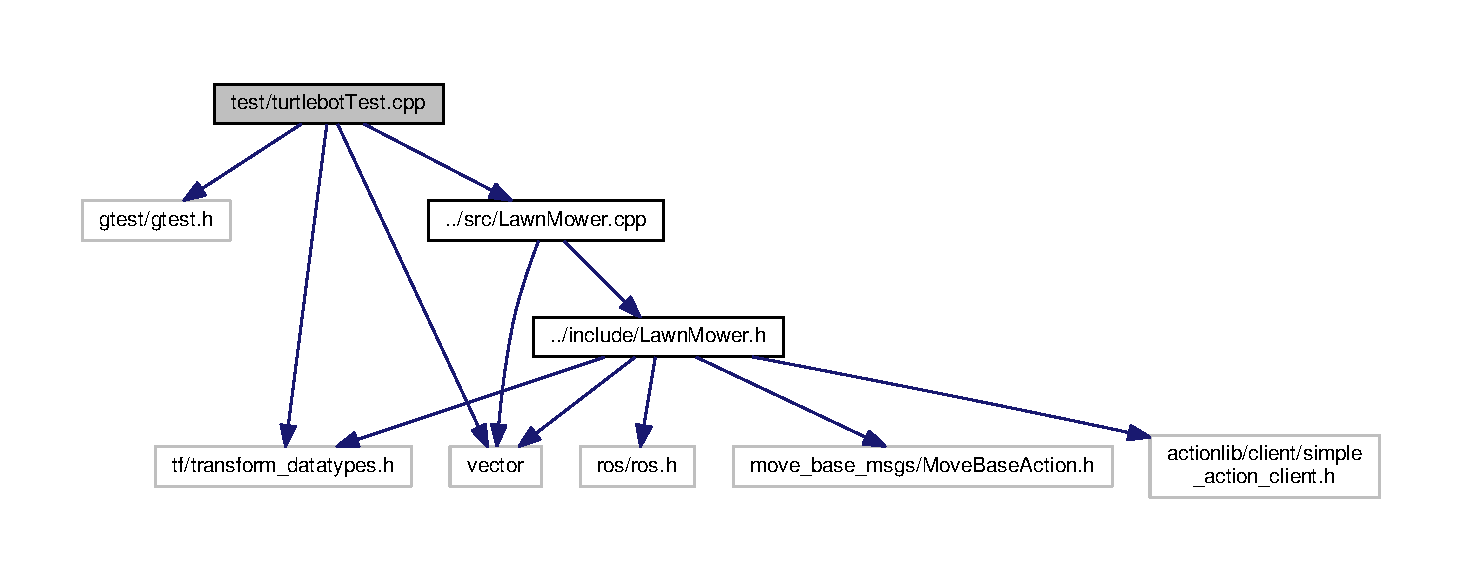
\includegraphics[width=350pt]{turtlebotTest_8cpp__incl}
\end{center}
\end{figure}
\subsection*{Functions}
\begin{DoxyCompactItemize}
\item 
\hyperlink{turtlebotTest_8cpp_aec20688b3dc0a2ca678c90ff98b8db39}{T\-E\-S\-T} (Quaternion\-Conversion, Correct\-Quaternion\-Calculation1)
\item 
\hyperlink{turtlebotTest_8cpp_a8b377cf4e80009e38990da523af77bc1}{T\-E\-S\-T} (Quaternion\-Conversion, Correct\-Quaternion\-Calculation2)
\item 
\hyperlink{turtlebotTest_8cpp_a965b0d14a8ee54b0c9f316c6864b98e7}{T\-E\-S\-T} (Quaternion\-Conversion, Correct\-Quaternion\-Calculation3)
\item 
\hyperlink{turtlebotTest_8cpp_a5ed6292138d3c7816d69c194eca9bd5c}{T\-E\-S\-T} (Quaternion\-Conversion, Correct\-Quaternion\-Calculation4)
\item 
\hyperlink{turtlebotTest_8cpp_a5adc1bc95493d5940d18e79ced656697}{T\-E\-S\-T} (Path\-Coordinates, get\-Path\-X\-Coordinate)
\item 
\hyperlink{turtlebotTest_8cpp_a1db8072bb01b9f201793cc28ba35989b}{T\-E\-S\-T} (Path\-Coordinates, get\-Path\-Y\-Coordinate)
\item 
\hyperlink{turtlebotTest_8cpp_a97ea4c2dda9469506e01ff1d61fbfc5d}{T\-E\-S\-T} (Path\-Coordinates, get\-Path\-Angle\-Pose)
\item 
int \hyperlink{turtlebotTest_8cpp_a3c04138a5bfe5d72780bb7e82a18e627}{main} (int argc, char $\ast$$\ast$argv)
\end{DoxyCompactItemize}


\subsection{Detailed Description}
File contains tests for the \hyperlink{classLawnMower}{Lawn\-Mower} class. \begin{DoxyAuthor}{Author}
Christian Ramos 
\end{DoxyAuthor}
\begin{DoxyDate}{Date}
10 May 2017 This file tests the \hyperlink{classLawnMower}{Lawn\-Mower} class member functions. Member functions that do not have return parameters are not tested, instead visual inspection is performed on this functions using R\-O\-S\-\_\-\-I\-N\-F\-O messages in the source code in order to provide the user a sense of parameters confidence while running the simulation.
\end{DoxyDate}
\begin{DoxySeeAlso}{See Also}
\href{https://github.com/traviezo/turtlebot_lawn_mower}{\tt https\-://github.\-com/traviezo/turtlebot\-\_\-lawn\-\_\-mower} 
\end{DoxySeeAlso}


\subsection{Function Documentation}
\hypertarget{turtlebotTest_8cpp_a3c04138a5bfe5d72780bb7e82a18e627}{\index{turtlebot\-Test.\-cpp@{turtlebot\-Test.\-cpp}!main@{main}}
\index{main@{main}!turtlebotTest.cpp@{turtlebot\-Test.\-cpp}}
\subsubsection[{main}]{\setlength{\rightskip}{0pt plus 5cm}int main (
\begin{DoxyParamCaption}
\item[{int}]{argc, }
\item[{char $\ast$$\ast$}]{argv}
\end{DoxyParamCaption}
)}}\label{turtlebotTest_8cpp_a3c04138a5bfe5d72780bb7e82a18e627}

\begin{DoxyCode}
100 \{
101   ros::init(argc, argv, \textcolor{stringliteral}{"turtlebotTest"});
102   testing::InitGoogleTest(&argc, argv);
103   \textcolor{keywordflow}{return} RUN\_ALL\_TESTS();
104 \}
\end{DoxyCode}
\hypertarget{turtlebotTest_8cpp_aec20688b3dc0a2ca678c90ff98b8db39}{\index{turtlebot\-Test.\-cpp@{turtlebot\-Test.\-cpp}!T\-E\-S\-T@{T\-E\-S\-T}}
\index{T\-E\-S\-T@{T\-E\-S\-T}!turtlebotTest.cpp@{turtlebot\-Test.\-cpp}}
\subsubsection[{T\-E\-S\-T}]{\setlength{\rightskip}{0pt plus 5cm}T\-E\-S\-T (
\begin{DoxyParamCaption}
\item[{Quaternion\-Conversion}]{, }
\item[{Correct\-Quaternion\-Calculation1}]{}
\end{DoxyParamCaption}
)}}\label{turtlebotTest_8cpp_aec20688b3dc0a2ca678c90ff98b8db39}

\begin{DoxyCode}
44 \{
45   \hyperlink{classLawnMower}{LawnMower} lawnMowerBot;
46   tf::Quaternion q;
47   q.setRPY(0.0, 0.0, 0.0);
48   EXPECT\_EQ(q, lawnMowerBot.\hyperlink{classLawnMower_a97a31ca30db64496d5a85b4218f69cab}{quaternionCalculation}(0.0));
49 \}
\end{DoxyCode}
\hypertarget{turtlebotTest_8cpp_a8b377cf4e80009e38990da523af77bc1}{\index{turtlebot\-Test.\-cpp@{turtlebot\-Test.\-cpp}!T\-E\-S\-T@{T\-E\-S\-T}}
\index{T\-E\-S\-T@{T\-E\-S\-T}!turtlebotTest.cpp@{turtlebot\-Test.\-cpp}}
\subsubsection[{T\-E\-S\-T}]{\setlength{\rightskip}{0pt plus 5cm}T\-E\-S\-T (
\begin{DoxyParamCaption}
\item[{Quaternion\-Conversion}]{, }
\item[{Correct\-Quaternion\-Calculation2}]{}
\end{DoxyParamCaption}
)}}\label{turtlebotTest_8cpp_a8b377cf4e80009e38990da523af77bc1}

\begin{DoxyCode}
52 \{
53   \hyperlink{classLawnMower}{LawnMower} lawnMowerBot;
54   tf::Quaternion q;
55   q.setRPY(0.0, 0.0, M\_PI);
56   EXPECT\_EQ(q, lawnMowerBot.\hyperlink{classLawnMower_a97a31ca30db64496d5a85b4218f69cab}{quaternionCalculation}(180.0));
57 \}
\end{DoxyCode}
\hypertarget{turtlebotTest_8cpp_a965b0d14a8ee54b0c9f316c6864b98e7}{\index{turtlebot\-Test.\-cpp@{turtlebot\-Test.\-cpp}!T\-E\-S\-T@{T\-E\-S\-T}}
\index{T\-E\-S\-T@{T\-E\-S\-T}!turtlebotTest.cpp@{turtlebot\-Test.\-cpp}}
\subsubsection[{T\-E\-S\-T}]{\setlength{\rightskip}{0pt plus 5cm}T\-E\-S\-T (
\begin{DoxyParamCaption}
\item[{Quaternion\-Conversion}]{, }
\item[{Correct\-Quaternion\-Calculation3}]{}
\end{DoxyParamCaption}
)}}\label{turtlebotTest_8cpp_a965b0d14a8ee54b0c9f316c6864b98e7}

\begin{DoxyCode}
60 \{
61   \hyperlink{classLawnMower}{LawnMower} lawnMowerBot;
62   tf::Quaternion q;
63   q.setRPY(0.0, 0.0, -(M\_PI/2));
64   EXPECT\_EQ(q, lawnMowerBot.\hyperlink{classLawnMower_a97a31ca30db64496d5a85b4218f69cab}{quaternionCalculation}(-90.0));
65 \}
\end{DoxyCode}
\hypertarget{turtlebotTest_8cpp_a5ed6292138d3c7816d69c194eca9bd5c}{\index{turtlebot\-Test.\-cpp@{turtlebot\-Test.\-cpp}!T\-E\-S\-T@{T\-E\-S\-T}}
\index{T\-E\-S\-T@{T\-E\-S\-T}!turtlebotTest.cpp@{turtlebot\-Test.\-cpp}}
\subsubsection[{T\-E\-S\-T}]{\setlength{\rightskip}{0pt plus 5cm}T\-E\-S\-T (
\begin{DoxyParamCaption}
\item[{Quaternion\-Conversion}]{, }
\item[{Correct\-Quaternion\-Calculation4}]{}
\end{DoxyParamCaption}
)}}\label{turtlebotTest_8cpp_a5ed6292138d3c7816d69c194eca9bd5c}

\begin{DoxyCode}
68 \{
69   \hyperlink{classLawnMower}{LawnMower} lawnMowerBot;
70   tf::Quaternion q;
71   q.setRPY(0.0, 0.0, (M\_PI/2));
72   EXPECT\_EQ(q, lawnMowerBot.\hyperlink{classLawnMower_a97a31ca30db64496d5a85b4218f69cab}{quaternionCalculation}(90.0));
73 \}
\end{DoxyCode}
\hypertarget{turtlebotTest_8cpp_a5adc1bc95493d5940d18e79ced656697}{\index{turtlebot\-Test.\-cpp@{turtlebot\-Test.\-cpp}!T\-E\-S\-T@{T\-E\-S\-T}}
\index{T\-E\-S\-T@{T\-E\-S\-T}!turtlebotTest.cpp@{turtlebot\-Test.\-cpp}}
\subsubsection[{T\-E\-S\-T}]{\setlength{\rightskip}{0pt plus 5cm}T\-E\-S\-T (
\begin{DoxyParamCaption}
\item[{Path\-Coordinates}]{, }
\item[{get\-Path\-X\-Coordinate}]{}
\end{DoxyParamCaption}
)}}\label{turtlebotTest_8cpp_a5adc1bc95493d5940d18e79ced656697}

\begin{DoxyCode}
76 \{
77   \hyperlink{classLawnMower}{LawnMower} lawnMowerBot;
78   std::vector<double> \hyperlink{turtlebot__lawn__mower_8cpp_ab924092e01ea1007f9b6d88bc3d9c723}{xCoordinates} \{ 0.25, 0.25,  2.75,  2.75, -1.25, -1.25,  3.25, 3.25, -1.25
      , -1.25,  3.25, 3.25, -1.25, -1.25,  3.25, 3.25, -1.25, -1.25,  3.25,  3.25, -0.5, -1.25, 3.25,  3.25\};
79   lawnMowerBot.\hyperlink{classLawnMower_a522dfba30f16929bbb4fa60af11771b3}{setPathX}(\hyperlink{turtlebot__lawn__mower_8cpp_ab924092e01ea1007f9b6d88bc3d9c723}{xCoordinates});
80   EXPECT\_EQ(2.75, lawnMowerBot.\hyperlink{classLawnMower_a989d400596032888d1e063dc289768b2}{getPathXCoordinate}()->at(3));
81 \}
\end{DoxyCode}
\hypertarget{turtlebotTest_8cpp_a1db8072bb01b9f201793cc28ba35989b}{\index{turtlebot\-Test.\-cpp@{turtlebot\-Test.\-cpp}!T\-E\-S\-T@{T\-E\-S\-T}}
\index{T\-E\-S\-T@{T\-E\-S\-T}!turtlebotTest.cpp@{turtlebot\-Test.\-cpp}}
\subsubsection[{T\-E\-S\-T}]{\setlength{\rightskip}{0pt plus 5cm}T\-E\-S\-T (
\begin{DoxyParamCaption}
\item[{Path\-Coordinates}]{, }
\item[{get\-Path\-Y\-Coordinate}]{}
\end{DoxyParamCaption}
)}}\label{turtlebotTest_8cpp_a1db8072bb01b9f201793cc28ba35989b}

\begin{DoxyCode}
84 \{
85   \hyperlink{classLawnMower}{LawnMower} lawnMowerBot;
86   std::vector<double> \hyperlink{turtlebot__lawn__mower_8cpp_a2fdc9aef0350032e97be2faac7fc0ec8}{yCoordinates} \{ 4.25, 3.75,  3.75,  3.25,  3.25,  2.75,  2.75, 2.25,  2.25
      ,  1.75,  1.75, 1.25,  1.25,  0.75,  0.75, 0.25,  0.25, -0.25, -0.25,  -0.5, -1.5, -0.25, 4.25,  4.25\};
87   lawnMowerBot.\hyperlink{classLawnMower_aa623d7ab5e162524a7c3ee9fe4de8fe1}{setPathY}(\hyperlink{turtlebot__lawn__mower_8cpp_a2fdc9aef0350032e97be2faac7fc0ec8}{yCoordinates});
88   EXPECT\_EQ(3.25, lawnMowerBot.\hyperlink{classLawnMower_a3def1589d73101f642f7465ec740762d}{getPathYCoordinate}()->at(3));
89 \}
\end{DoxyCode}
\hypertarget{turtlebotTest_8cpp_a97ea4c2dda9469506e01ff1d61fbfc5d}{\index{turtlebot\-Test.\-cpp@{turtlebot\-Test.\-cpp}!T\-E\-S\-T@{T\-E\-S\-T}}
\index{T\-E\-S\-T@{T\-E\-S\-T}!turtlebotTest.cpp@{turtlebot\-Test.\-cpp}}
\subsubsection[{T\-E\-S\-T}]{\setlength{\rightskip}{0pt plus 5cm}T\-E\-S\-T (
\begin{DoxyParamCaption}
\item[{Path\-Coordinates}]{, }
\item[{get\-Path\-Angle\-Pose}]{}
\end{DoxyParamCaption}
)}}\label{turtlebotTest_8cpp_a97ea4c2dda9469506e01ff1d61fbfc5d}

\begin{DoxyCode}
92 \{
93   \hyperlink{classLawnMower}{LawnMower} lawnMowerBot;
94   std::vector<double> \hyperlink{turtlebot__lawn__mower_8cpp_a06c7ee380c5c4448f42b667fb3a645c4}{anglePose} \{-90.0,  0.0, -90.0, 180.0, -90.0,   0.0, -90.0,  180, -90.0,   0.
      0, -90.0,  180, -90.0,   0.0, -90.0,  180, -90.0,   0.0, -90.0, 180.0, 90.0,   0.0,  0.0, 180.0\};
95   lawnMowerBot.\hyperlink{classLawnMower_a05dbed29e3ee522d845c8fbb9fe4b986}{setAnglePose}(\hyperlink{turtlebot__lawn__mower_8cpp_a06c7ee380c5c4448f42b667fb3a645c4}{anglePose});
96   EXPECT\_EQ(180, lawnMowerBot.\hyperlink{classLawnMower_aec7ea498bca8e6092d7d8ae1f90417c3}{getPathAnglePose}()->at(3));
97 \}
\end{DoxyCode}

%--- End generated contents ---

% Index
\newpage
\phantomsection
\addcontentsline{toc}{chapter}{Index}
\printindex

\end{document}
